\documentclass{standalone}
\usepackage{graphicx}	
\usepackage{amssymb, amsmath, amsthm}
\usepackage{color}

\usepackage{tikz}
\usetikzlibrary{intersections, backgrounds}

\definecolor{light}{RGB}{220, 188, 188}
\definecolor{mid}{RGB}{185, 124, 124}
\definecolor{dark}{RGB}{143, 39, 39}
\definecolor{highlight}{RGB}{180, 31, 180}
\definecolor{gray10}{gray}{0.1}
\definecolor{gray20}{gray}{0.2}
\definecolor{gray30}{gray}{0.3}
\definecolor{gray40}{gray}{0.4}
\definecolor{gray60}{gray}{0.6}
\definecolor{gray70}{gray}{0.7}
\definecolor{gray80}{gray}{0.8}
\definecolor{gray90}{gray}{0.9}
\definecolor{gray60}{gray}{0.95}

\begin{document}

\begin{tikzpicture}[scale=0.45, thick]

\begin{scope}[shift={(0, 0)}]
  \draw[white] (-7, -7) rectangle (7, 5);
    
  \begin{scope}
    \clip (-7, -7) rectangle (7, 5);
        \node at (0, 0) {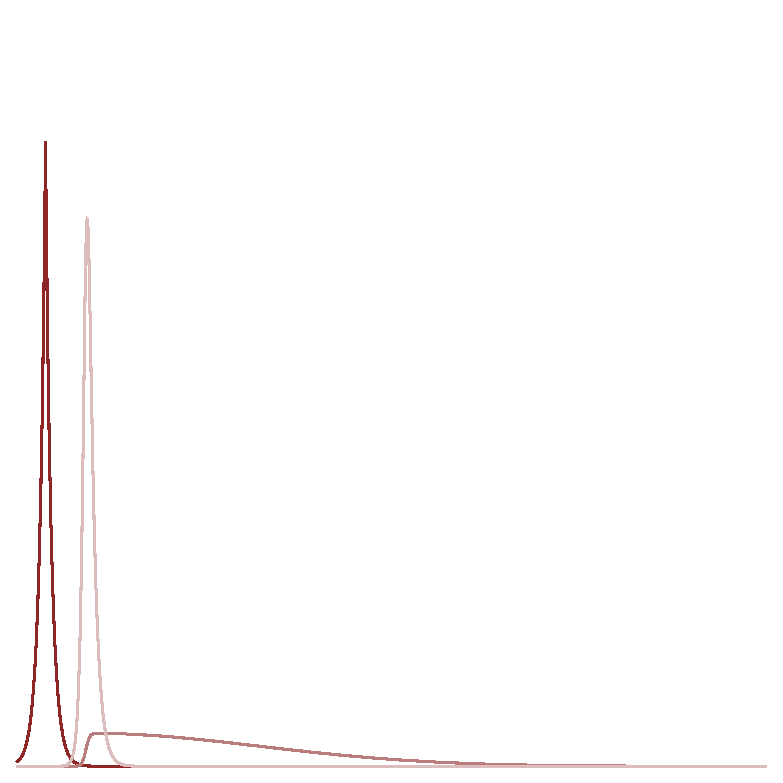
\includegraphics[width=4.5cm]{laplace_outer.eps}};
  \end{scope}
  
  \node[dark] at (-4.5, 4) { Prior };
  \node[mid] at (2, -4.25) { Likelihood };
  \node[light] at (-2, -3) { Posterior };
  
  \draw [<->, >=stealth, line width=1] (-5 - 0.025, -5) -- +(10, 0);
  \node[] at (0, -6) { $\theta_{k}$ };
\end{scope}

\end{tikzpicture}

\end{document}  